
\documentclass[paper=a4, fontsize=11pt]{scrartcl} % A4 paper and 11pt font size
\newcommand{\horrule}[1]{\rule{\linewidth}{#1}}
\usepackage{ctex}
\usepackage{indentfirst}
\usepackage[T1]{fontenc} % Use 8-bit encoding that has 256 glyphs
\usepackage{fourier} % Use the Adobe Utopia font for the document - comment this line to return to the LaTeX default
\usepackage[english]{babel} % English language/hyphenation
\usepackage{amsmath,amsfonts,amsthm} % Math packages

\usepackage{lipsum} % Used for inserting dummy 'Lorem ipsum' text into the template

\usepackage{sectsty} % Allows customizing section commands
\allsectionsfont{\centering \normalfont\scshape} % Make all sections centered, the default font and small caps

\usepackage{fancyhdr} % Custom headers and footers
\pagestyle{fancyplain} % Makes all pages in the document conform to the custom headers and footers
\fancyhead[c]{\kaishu 油滴实验的讨论} % No page header - if you want one, create it in the same way as the footers below
\fancyfoot[L]{} % Empty left footer
\fancyfoot[C]{\thepage} % Empty center footer
\fancyfoot[R]{} % Page numbering for right footer
\renewcommand{\headrulewidth}{0pt} % Remove header underlines
\renewcommand{\footrulewidth}{0pt} % Remove footer underlines
\setlength{\headheight}{13.6pt} % Customize the height of the header

\numberwithin{equation}{section} % Number equations within sections (i.e. 1.1, 1.2, 2.1, 2.2 instead of 1, 2, 3, 4)
\numberwithin{figure}{section} % Number figures within sections (i.e. 1.1, 1.2, 2.1, 2.2 instead of 1, 2, 3, 4)
\numberwithin{table}{section} % Number tables within sections (i.e. 1.1, 1.2, 2.1, 2.2 instead of 1, 2, 3, 4)


%----------------------------------------------------------------------------------------
%	TITLE SECTION
%----------------------------------------------------------------------------------------

\title{	
\normalfont \normalsize 
\textsc{Shanghai Jiao Tong University} \\ [25pt] % Your university, school and/or department name(s)
\horrule{0.5pt} \\[0.4cm] % Thin top horizontal rule
\huge \kaishu 油滴实验的讨论 \\ % The assignment title
\horrule{2pt} \\[0.5cm] % Thick bottom horizontal rule
}

\author{\kaishu 冯伟琪} % Your name

\date{\normalsize\today} % Today's date or a custom date

\begin{document}

\maketitle % Print the title
\section{\kaishu 油滴实验简介}
\kaishu 
油滴实验是由美国科学家密立根在1909用来测量单个电子所带电荷量的实验。下面介绍一种动态测量法,其主要原理是通过分别测量油滴经过电场和不经过电场的速度以及利用最后的平衡力学方程来求取电子所带的电荷量。实验装置简图如\ref{fig:0} 所示。

\begin{figure}[!htp]
	\centering
	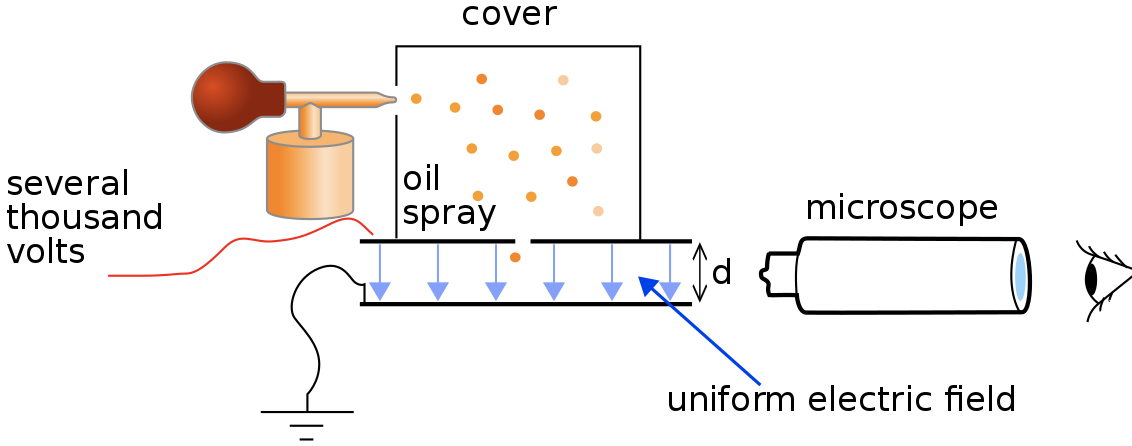
\includegraphics[width=0.7\textwidth]{fig0}
	\caption{\kaishu 油滴实验装置图}
	\label{fig:0}
\end{figure}

在喷雾的过程中,部分油滴可能会因与喷嘴的摩擦和带上电荷。值得注意的是所有的实验测量都是在一个选择好的油滴上进行的。

首先我们考虑油滴在电场不存在的下落过程,其受力分析如图\ref{fig:1}左图所示。油滴最终会达到稳定速度$v_1$,在该状态下油滴受到油滴本身的重力$F_{w}$、浮力$F_{b}$,阻力$F_{d}$。并且我们可以得到如下的力学方程组:

\begin{equation}
	\begin{cases}
		F_w = mg = \dfrac{4}{3}\pi r^3 \rho_{oil}g\\
		F_b = \dfrac{4}{3} \pi r^3 \rho_{air} g\\
		F_d = 6\pi r \eta v_1\\
		F_w=F_b+F_d
	\end{cases}
	\label{eq:0}
\end{equation}

在本实验过程中,我们可以将油滴当做球体来处理。并且对于空气阻力,我们可以采用斯托克斯定律做处理。根据力学方程组\eqref{eq:0},我们可以解得难以直接测量的半径$r$。

\begin{equation}
	r = \sqrt{\frac{9\eta v_1}{2g(\rho_{oil}-\rho_{air})}}
	\label{eq:1}
\end{equation}
\begin{figure}[!htp]
	\centering
	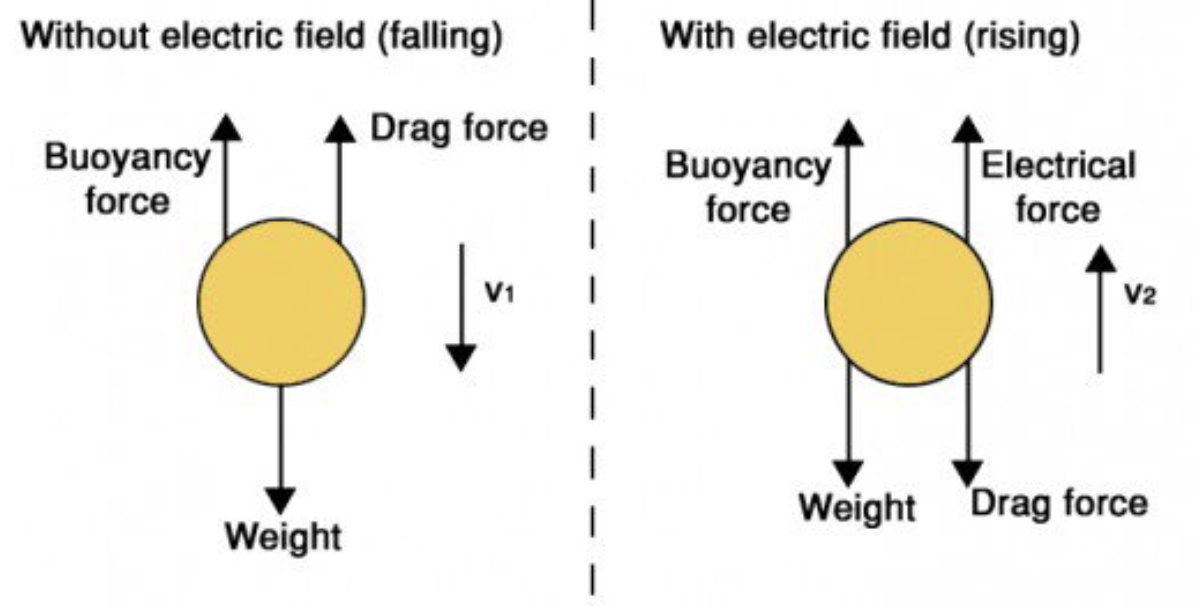
\includegraphics[width=0.7\textwidth]{1.png}
	\caption{\kaishu 油滴受力示意图}
	\label{fig:1}
\end{figure}

下面考虑第二种情况,油滴在电场中达到最后稳定速度$v_2$的过程。若两极板施加电压相对较大,其会如图\ref{fig:1}右图所示向上运动。我们可知其在该状态下除了第一种情况所受到的三种力以外,还受到电场力$F_e$。我们可以由此得到力学方程组\eqref{eq:2}

\begin{equation}
	\begin{cases}
		E = \dfrac{V}{d}\\
		F_w = mg = \dfrac{4}{3}\pi r^3 \rho_{oil}g\\
		F_b = \dfrac{4}{3}\pi r^3 \rho_{air} g\\
		F_d = 6\pi r \eta v_2\\
		F_e = qE\\
		F_w+F_d=F_e+F_b
	\end{cases}
	\label{eq:2}
\end{equation}

$V$为我们在极板两级施加的电压,$d$为两极板之间的距离。再利用公式\eqref{eq:2} 我们已经得到的半径$r$,我们可以得到油滴所带的带电量$q$。

\begin{equation}
	\centering
	q=\dfrac{9\pi d(v_1+v_2)}{V}\sqrt{\dfrac{2\eta^3 v_1}{g(\rho_{oil}-\rho_{air})}}
	\label{eq:3}
\end{equation}

我们可以利用这种方法,选择不同油滴重复上述实验。我们可以发现所测得的电量均为某一具体数值的整数倍,而这个数值就是一个电子的电荷量$e$。

\section{\kaishu 相关实验参数讨论}

通过分析上述实验过程,我们可以发现油滴实验的原理并不复杂,是一种简单有效测量电子电荷量的实验。但是在实际测量过程中,我们往往会遇到很多现实中测量的难题。为了解决这些问题,我们需要将实验参数进行合理设计。

\subsection{\kaishu 观察室参数}
根据实验原理,我们可以发现所有的速度测量都是在同一个油滴上进行。在实验过程中,我们在众多油滴当中锁定某一个具体油滴是非常困难的。同时为了测量两个状态的稳定速度$v_1$和$v_2$,我们还需要测量油滴运动一段距离所需要的时间。这些都需要我们能够在整个实验流程中清楚地观察到油滴的运动状态。

一个简单可行的解决方法是在不超过实验器材体积参数的条件下,适当增大观察室的视野,这样可以使我们能够更准确地观察油滴的运动情况。

\subsection{\kaishu 油滴选择}
选择好一个恰当大小的油滴是非常重要的。如果选择的油滴太小,布朗运动效果明显,测量不准确;如果选择的油滴太大,一般来说带电量较多,下落速度较快,不容易准确测量。

带电量较多对实验数据处理也存在不利影响,当油滴所带的电荷量较大时,我们难以确定其电子所带的基本电荷量。因为我们发现无论是整除$n$或者$n+1$或者$n-1$,计算的基本电荷量结果都非常接近。

我们应该在实验中选择质量适中,携带10倍左右元电荷电量的油滴。(改变油滴所带电荷量可以利用其它放射源手工改变)。根据经验表明,平衡电压在200$V$左右,并且在20s内左右时间内匀速下降2mm的油滴,其大小和带电量都比较适中。

\subsection{\kaishu 极板距离的选定}
选择恰当的极板距离非常重要。其不仅影响到电场中电场强度的大小,同时还影响油滴能否做匀速直线运动。下面我们先考虑后者的影响。

我们可以将极板距离分为三部分,第一部分为反应距离,第二部分为测量距离,第三部分为安全距离。我们需要保证在反应距离过程中油滴已经做匀速直线运动。事实上,反应距离理论计算相对较难,但我们可以大约估计其所需要的时间。下面我们近似量化计算(忽略空气浮力)

\begin{displaymath}
\centering
mg-q\dfrac{V}{d}-6\pi r \eta v = m\dfrac{dv}{dt}
\end{displaymath}

解得:

\begin{displaymath}
	\centering
v = A + Ce^{-kt}
\end{displaymath}

其中$A=\dfrac{mg-q\dfrac{V}{d}}{6\pi r \eta}$,$K=\dfrac{6\pi r \eta}{m}$,$C$为待定常数,由初始条件确定。

初始条件为:电场力为0和初始速度为0。带入初始条件,解得速度$v$的解析式:

\begin{displaymath}
	v=\dfrac{g}{k}(1-e^{-kt})
\end{displaymath}

经分析可知$\dfrac{g}{k}$即为油滴最终达到的稳定速度。取$e^{-kt}\leq 0.0001$。这时速度已经达到匀速运动的$99.99\%$,可认为已经匀速。此时求得:

\begin{displaymath}
	t \geq \dfrac{4}{k} \ln{10}=4\dfrac{l}{gt_g}\ln{10}
	\quad
	l_1 \leq vt=\dfrac{l}{t_g}t
\end{displaymath}

可知$l$为为了计算速度所规定的测量距离,$t_g$则为油滴在该过程中下落的时间,$l_1$则为提到的反应距离。为了便于观察和计算,我们不妨假定能通过调节两极板间电压和极板间距离来控制测量距离和下落时间。不妨假定$l=2mm$,$t_g=15s$,重力加速度$g=9.8m/s^2$。

\begin{displaymath}
	t \geq 1.25\times 10^{-4}s
	\quad
	l_1\leq 1.67\times 10^{-5} mm
\end{displaymath}

由计算可知$l_1$相对而言很小,完全可以通过改变极板距离来确保其做匀速直线运动。选择测量距离的位置也需要多加考虑,如果太靠近上级板,小孔附近有气流,电场也不均匀,会影响结果;如果太靠近下级板,测量完时间$t_g$后,油滴容易丢失,不利于后面上升时间的测定。

\subsection{\kaishu 极板电压的选择}

两极板电压选择十分关键,因为它直接影响到了油滴在测量距离过程中运动所需要的时间。如果时间过短,其测量过程中误差较大。如果时间太长,则整个实验时间会显著增加。下面我们简单计算两极板所需电压大小。由上一小节可知,我们认为$t_g=15s$较为理想,并且我们假定极板距离为$d=5mm$,油滴带电量为$10e$,$\eta_{t=20^\circ}=1.83\times 10^{-5}kg\cdot m^{-1} \cdot s^{-1}$,$\rho_{oil}=981kg\cdot m^{-3} $,$\rho_{air}=1.293kg\cdot m^{-3}$,其余参数(除电压)与上一小节假设完全相同

则将等式\eqref{eq:3}变形可得

\begin{displaymath}
		V=\dfrac{9\pi d(v_1+v_2)}{q}\sqrt{\dfrac{2\eta^3 v_1}{g(\rho_{oil}-\rho_{air})}}
\end{displaymath}

代入数据计算的

\begin{displaymath}
	V=307.40V
\end{displaymath}

由于不同油滴的带电量可能会有所差异,所以我们认为两极板间电压应大致介于300$V$和500$V$之间。






\section{\kaishu 油滴实验的巧妙之处}
油滴实验的巧妙之处在于把电子所带的电荷量这种极其微小的微观物理量,通过巧妙的实验设计,转化为测量油滴的下落和上升速度。如果选择的实验参数和实验仪器合理有效,我们可以较为准确的测量出油滴在在反应距离内运动的时间。并且根据求得的时间,求得油滴匀速运动的速度。最终,我们通过对实验的数据分析,可以得到一个电子所带的电荷量。

相较于其他实验,油滴实验原理简单,实验思路清晰,可重复性强。但是在实际实验过程中,实验参数的选定还是需要一番仔细的斟酌。








\end{document}